% 02-analiza-sustava.tex - USPOREDBA SUSTAVA I NAPREDNI PRISTUPI

\section{USPOREDBA POSTOJEĆIH SUSTAVA I NAPREDNI UPRAVLJAČKI PRISTUPI}
\label{sec:analiza_sustava}

Kako bi se teorijski koncepti upravljanja silom primijenili u kliničkim uvjetima, razvijeni su različiti eksperimentalni i komercijalni sustavi. U ovom poglavlju dan je pregled konkretnih robotskih rješenja iz literature te se analiziraju napredne upravljačke strategije koje predstavljaju znanstveni vrhunac u području robotske ehografije.

\subsection{Usporedna analiza konkretnih sustava iz literature}
U tablici \ref{tab:usporedba_sustava} prikazana je detaljna usporedba triju reprezentativnih robotskih sustava koji se koriste za ultrazvučno snimanje različitih organa, sa svim njihovim tehničkim specifikacijama, vrstama senzora i razinama autonomije prema LORA (engl. \textit{Level of Robot Autonomy}) klasifikaciji \cite{vonhaxthausen2021medical}.

\begin{table}[H]
\centering
\caption{Usporedna analiza konkretnih robotskih ultrazvučnih sustava.}
\label{tab:usporedba_sustava}
\begin{tabularx}{\textwidth}{p{0.18\textwidth} X X X}
\toprule
\textbf{Parametar} & \textbf{HaptiScan \cite{conti2010interface}} & \textbf{Breast-Scanning \cite{ieee2023full}} & \textbf{Thyroid-Scanning \cite{li2026robotic}} \\
\midrule
\textbf{Korišteni robot} & Universal Robots UR5 (6-DoF) & KUKA LBR Med7 (7-DoF) & UFACTORY xArm6 (6-DoF) \\
\textbf{Vrsta senzora} & 6-osni F/T senzor na vrhu + Phantom Omni master & Integrirani senzori momenta u zglobovima + F/T senzor & 6-osni F/T senzor na vrhu robota \\
\textbf{Tip upravljanja} & Admitancijsko upravljanje s haptičkim feedbackom & Hibridno force-velocity (admitancijsko) upravljanje & Admitancijsko upravljanje drugog reda (MSD model) \\
\textbf{Cilj snimanja} & Opća dijagnostika na daljinu (teleoperacija) & Skeniranje cijele površine dojke (rak dojke) & Skeniranje štitnjače kod pacijenata \\
\textbf{Razina autonomije} & Poluautonomno (LORA 2) & Visoka autonomija (LORA 4) & Poluautonomno (LORA 3) \\
\textbf{Ograničenja} & Kašnjenje signala (latencija), zamor operatera & Visoka cijena KUKA LBR robota, složena kalibracija momenta & Osjetljivost na brza gibanja štitnjače pri gutanju \\
\bottomrule
\end{tabularx}
\end{table}

Kao primjer visokoautonomnog sustava iz Tablice \ref{tab:usporedba_sustava}, Slika \ref{fig:breast_scan} ilustrira eksperimentalni postav s KUKA LBR Med7 manipulatorom, integriranim senzorima sile i ultrazvučnom sondom, namijenjen za automatsku 3D rekonstrukciju tkiva dojke \cite{ieee2023full}.

\begin{figure}[H]
    \centering
    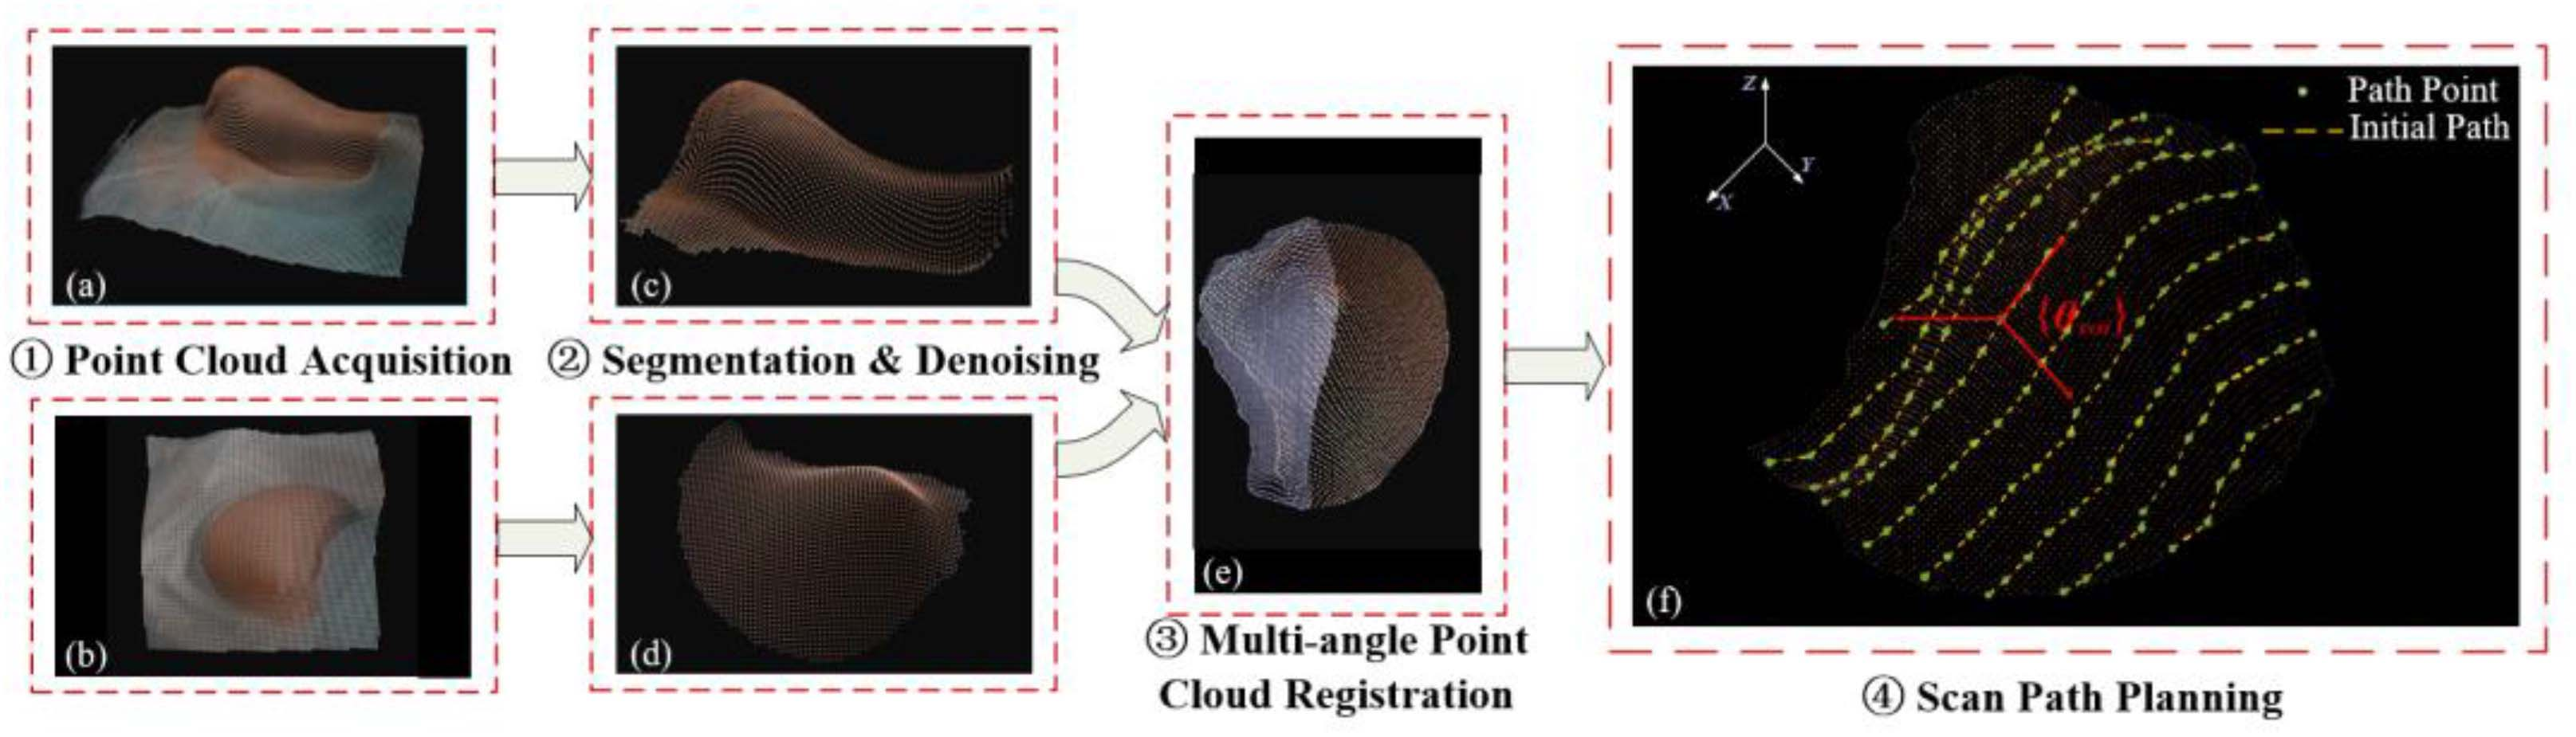
\includegraphics[width=0.65\textwidth]{figures/breast_scan_4_3}
    \caption{Eksperimentalni robotski sustav visoke autonomije za automatsko skeniranje dojke temeljen na KUKA LBR Med7 manipulatoru (prilagođeno iz \cite{ieee2023full}).}
    \label{fig:breast_scan}
\end{figure}

\subsection{Vizualno vođeno upravljanje silom (Image-Guided Control)}
Jedan od najvećih iskoraka u robotskom ultrazvuku je integracija vizualnih informacija iz same ultrazvučne slike u zatvorenu petlju upravljanja silom. Umjesto održavanja konstantne sile bez obzira na kvalitetu slike, ovi sustavi prilagođavaju ciljanu silu $F_d$ na temelju analize slike u realnom vremenu.
\begin{itemize}
    \item \textbf{Mape pouzdanosti (Confidence Maps):} Twente grupa \cite{twente2024comparison} razvija hibridni pristup u kojem se analizira akustička sjena i gubitak signala. Ako sustav detektira loš kontakt (npr. zrak između sonde i kože), kontroler povećava silu dok se ne uspostavi akustički prozor.
    \item \textbf{Vizualni servo-sustavi (Visual Servoing):} Akbari i suradnici \cite{akbari2021robotic} koriste strojno učenje (SVM klasifikator) za procjenu kvalitete slike. Kad indeks kvalitete padne ispod zadane granice, sila se dinamički korigira. IEEE RA-L rad iz 2025. \cite{ieee2025smooth} i SAGE rad iz 2026. \cite{sage2026explicit} pokazuju da vizualno vođeno upravljanje značajno poboljšava stabilnost signala i smanjuje pogreške pri prijelazima preko složenih geometrija.
\end{itemize}

\subsection{Upravljanje temeljeno na učenju (Learning-Based Control)}
Učenje u robotskom ultrazvuku koristi se za modeliranje složenih, nelinearnih interakcija koje je teško opisati klasičnim fizikalnim jednadžbama.
\begin{itemize}
    \item \textbf{Inverse Reinforcement Learning (IRL):} U radu \cite{ieee2024inverse} koristi se IRL kako bi robot naučio pravila skeniranja promatrajući iskusne liječnike. Robot uči funkciju nagrade (\textit{reward function}) koja balansira silu pritiska i brzinu gibanja, omogućujući prilagodbu krutosti u nesigurnim okolinama.
    \item \textbf{Reinforcement Learning (RL):} Autonomno skeniranje i optimizacija položaja sonde mogu se riješiti metodama dubokog pojačanog učenja \cite{ieee2021autonomic}. Kako bi se izbjegle opasnosti online učenja na ljudima, najnoviji pristupi koriste \textit{Offline Reinforcement Learning} \cite{ieee2025offline} za offline treniranje algoritama na simulatorima i datasetovima prije izravne primjene u klinici, osiguravajući adaptivnu impedanciju bez rizika za pacijenta.
\end{itemize}

\subsection{Prilagodljivo upravljanje silom (Adaptive Force Control)}
Strukturna svojstva ljudskog tijela variraju od mekih (trbuh) do vrlo tvrdih regija (rebra). Standardni admitancijski kontroleri s fiksnim parametrima ($M_d, B_d, K_d$) postaju nestabilni pri naglim promjenama krutosti okoline. Prilagodljivo (adaptivno) upravljanje silom rješava ovaj problem online procjenom krutosti tkiva $K_e$ i dinamičkim modificiranjem parametara prigušenja $B_d(t)$ \cite{jiang2024force, li2026robotic}. Na taj se način osigurava da sustav ostane stabilan i ne oscilira ni na tvrdim koštanim strukturama ni na mekom tkivu.

\subsection{Zajednička autonomija i multimodalno upravljanje}
Kombinacija različitih senzorskih modaliteta ključna je za visoke razine autonomije.
\begin{itemize}
    \item \textbf{Zajednička autonomija (Shared Autonomy):} Omogućuje podjelu uloga. Na primjer, liječnik kontrolira poziciju sonde na daljinu (teleoperacija), dok robot lokalno i autonomno održava normalnu orijentaciju sonde na površinu kože i konstantan pritisak od npr. 5 N, kompenzirajući sitne podrhtaje liječnikove ruke \cite{akbari2021robotic}.
    \item \textbf{Multimodalno upravljanje (Multimodal Control):} Koristi istovremenu fuziju sile, slike i vizualnih kamera za praćenje vanjske geometrije pacijenta. U radu \cite{ieee2025respiratory} prikazana je fuzija vizualnih i haptičkih podataka (engl. \textit{Vision-Haptic Fusion}) koja omogućuje trodimenzionalnu rekonstrukciju organa uz robusno praćenje disanja pacijenta.
\end{itemize}
